\subsection{Basic Vector Operations}
We have a few vector operations that are worth mentioning. We start with what are called ``unary" operators, or operations that only require a single input. Examples of unary operators on the real numbers are negation (i.e. turning $4$ into $-4$), or reciprocation (i.e. turning $4$ into $1/4$). The first unary operator we'll look at for vectors is \textbf{magnitude}.

\begin{definition}{Magnitude}
Let $\vcv$ be an $n$-dimensional vector, that is $\vcv=\bmat{v_1\\v_2\\ \vdots \\ v_n}$. Then the magnitude of $\vcv$ is: $$||\vcv||=\sqrt{v_1^2+v_2^2+\cdots+v_n^2}. $$
\end{definition}

\begin{exercise}{Magnitudes}
Find the magnitude for the following vectors:
\begin{enumerate}
\item $\vcv=(1,4)$
\vspace{1em}
\item $\vcu=(3,-2)$
\vspace{1em}
\item $\vca=(3,1,-2)$
\vspace{1em}
\item $\vcb=(6,2,-4,12)$
\end{enumerate}
\end{exercise}

A related definition is that of the \textbf{unit vector}. Technically you can think of this as a unary operation that takes a vector and returns the unit version of that vector.

\begin{definition}{Unit Vector}
We say that $\vcv$ is a \textbf{unit} vector if $||\vcv||=1$. We can find a unit vector that is parallel (has the same direction) of $\vcv$ by dividing $\vcv$ by its own magnitude. That is: $$\hat{v}=\frac{1}{||\vcv||}\vcv.$$
\end{definition}

\begin{definition}{Zero Vector}
We say that $\vcv$ is the \textbf{zero} vector if $||\vcv||=0$, and we write $\vcv=\vzero$.
\end{definition}

The second important unary operation is \textbf{negation}. 

\begin{definition}{Vector Negation}
Let $\vcv\in\bbr^n$, that is, $\vcv=\bmat{v_1\\v_2\\ \vdots \\ v_n}$. Then $-\vcv=\bmat{-v_1\\-v_2\\ \vdots \\ -v_n}$.
\end{definition}

Then that brings us into our second category of operations, ``binary" operators, or operators that require two inputs. Examples of binary operators on real numbers are addition, multiplication, etc. We see analogues for these for vectors in vector addition and scalar multiplication.

\begin{definition}{Vector Addition}
Let $\vcv$ and $\vcu$ be two vectors in $\bbr^n$. Then to add these two vectors, we add the corresponding coordinates. That is,
$$\vcv\pm \vcu=\bmat{v_1\\v_2\\ \vdots\\v_n}\pm\bmat{u_1\\u_2\\ \vdots\\u_n}=\bmat{v_1\pm u_1\\v_2\pm u_2\\ \vdots\\v_n\pm u_n}. $$
\end{definition}

\begin{definition}{Scalar Multiplication}
Given a vector $\vcv$ in $\bbr^n$ and a number $c$ in $\bbr$ (called a scalar), their product is defined by distributing the scalar to each coordinate of the vector. That is,
$$c\vcv=c\bmat{v_1\\v_2\\ \vdots\\v_n}=\bmat{cv_1\\cv_2\\ \vdots \\ c v_n}.$$
\end{definition}

The way we add vectors is ``timewise". Vectors are typically drawn as arrows with a length(magnitude) and direction. If we place the tail of the vector $\vcv=(x,y)$ on the origin, the tip of the arrow would land at the point $(x,y)$. 

\begin{center}
\begin{tikzpicture}[scale=.7, x=1cm, y=1cm, semitransparent]
	%\draw[step=1mm, line width=0.1mm, black!20!white] (0,0) grid (\width,\hauteur);
	%\draw[step=5mm, line width=0.2mm, black!90!white] (0,0) grid (\width,\hauteur);
	\draw[step=5cm, line width=0.5mm, black!90!white] (0,0) grid (\width,\hauteur);
	\draw[step=1cm, line width=0.2mm, black!50!white] (0,0) grid (\width,\hauteur);
	\draw[->, color=blue,line width=0.5mm](5,5)--(7.6,6);
	\node[color=blue] (v) at (6,6){$\vcv$};
	\draw[->, color=red, line width=0.5mm](5,5)--(7,3.6);
	\node[color=red] (u) at (5.6,3.8){$\vcu$};
	\end{tikzpicture}\end{center}

Geometrically, to add two vectors, we follow one, then follow the other. That is, we place them tail to tip:

\begin{center}
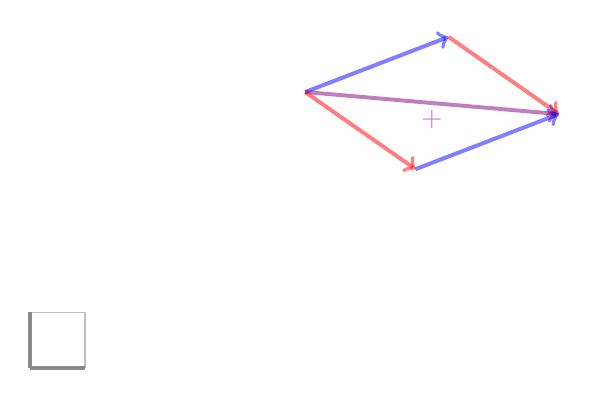
\begin{tikzpicture}[scale=.7, x=1cm, y=1cm, semitransparent]
	%\draw[step=1mm, line width=0.1mm, black!20!white] (0,0) grid (\width,\hauteur);
	%\draw[step=5mm, line width=0.2mm, black!90!white] (0,0) grid (\width,\hauteur);
	\draw[step=5cm, line width=0.5mm, black!90!white] (0,0) grid (\width,\hauteur);
	\draw[step=1cm, line width=0.2mm, black!50!white] (0,0) grid (\width,\hauteur);
	\draw[->, color=blue,line width=0.5mm](5,5)--(7.6,6);
	\node[color=blue] (v) at (6,6){$\vcv$};
	\draw[->, color=red, line width=0.5mm](7.6,6)--(9.6,4.6);
	\node[color=red] (u) at (8.5,6){$\vcu$};
	\draw[->,color=violet,line width=0.5mm](5,5)--(9.6,4.6);
	\node[color=violet](uv) at (7.3, 4.5){$\vcv+\vcu$};
	\draw[->, color=red, line width=0.5mm](5,5)--(7,3.6);
	\node[color=red] (u1) at (5.6,3.8){$\vcu$};
	\draw[->, color=blue,line width=0.5mm](7,3.6)--(9.6,4.6);
	\node[color=blue] (v1) at (8.5,3.5){$\vcv$};
	\end{tikzpicture}\\
	For a 3d example, look \href{https://www.geogebra.org/3d/kdfbhfvx}{here}.\end{center}

Note, commutativity holds! If we follow $\vcv$ first, then $\vcu$, we end up at the same spot as if we followed $\vcu$ first then $\vcv$. In fact, this makes a parallelogram. 

The vector drawn from the starting point to the ending point is exactly the sum of the two vectors. The difference of two vectors can be found from the same triangle as the sum:

\begin{center}
\begin{tikzpicture}[scale=.7, x=1cm, y=1cm, semitransparent]
	%\draw[step=1mm, line width=0.1mm, black!20!white] (0,0) grid (\width,\hauteur);
	%\draw[step=5mm, line width=0.2mm, black!90!white] (0,0) grid (\width,\hauteur);
	\draw[step=5cm, line width=0.5mm, black!90!white] (0,0) grid (\width,\hauteur);
	\draw[step=1cm, line width=0.2mm, black!50!white] (0,0) grid (\width,\hauteur);
	\draw[->, color=blue,line width=0.5mm](5,5)--(7.6,6);
	\node[color=blue] (v) at (6,6){$\vcv$};
	\draw[->, color=red, line width=0.5mm](5,5)--(7,3.6);
	\node[color=red] (u) at (5.6,3.8){$\vcu$};
	\draw[->, color=violet, line width=0.5mm](7.6,6)--(7,3.6);
	\node[color=violet] (w) at (8.6,4.5){$\vcw=\vcu-\vcv$};
	\end{tikzpicture}\\
	For a 3d example, look \href{https://www.geogebra.org/3d/zqhabgw9}{here}.\end{center}

Here, $\vcv+\vcw=\vcu$. Then it follows that $\vcu-\vcv=\vcw$. That is, the difference between two vectors is the vector that goes from the tip of the second (``negative") vector to the tip of the second (``positive") vector.

\index{Vector!Scalar Multiplication}To multiply a vector by a scalar, we just scale the vector. In other words, the magnitude of the vector increases or decreases. For example:
\begin{center}
\begin{tikzpicture}[scale=.5, x=1cm, y=1cm, semitransparent]
	%\draw[step=1mm, line width=0.1mm, black!20!white] (0,0) grid (\width,\hauteur);
	%\draw[step=5mm, line width=0.2mm, black!90!white] (0,0) grid (\width,\hauteur);
	\draw[step=5cm, line width=0.5mm, black!90!white] (0,0) grid (\width,\hauteur);
	\draw[step=1cm, line width=0.2mm, black!50!white] (0,0) grid (\width,\hauteur);
	\draw[->, color=red, line width=0.5mm](5,5)--(7,3.6);
	\node[color=red] (u) at (5.6,3.8){$\vcu$};
	\end{tikzpicture}
	\begin{tikzpicture}[scale=.5, x=1cm, y=1cm, semitransparent]
	%\draw[step=1mm, line width=0.1mm, black!20!white] (0,0) grid (\width,\hauteur);
	%\draw[step=5mm, line width=0.2mm, black!90!white] (0,0) grid (\width,\hauteur);
	\draw[step=5cm, line width=0.5mm, black!90!white] (0,0) grid (\width,\hauteur);
	\draw[step=1cm, line width=0.2mm, black!50!white] (0,0) grid (\width,\hauteur);
	\draw[->, color=red, line width=0.5mm](5,5)--(9,2.2);
	\node[color=red] (u) at (7,3){$2\vcu$};
	\end{tikzpicture}\end{center}

If that scalar is negative, the direction of the vector reverses! This is similar to how negative numbers go in the opposite direction of positive numbers along the number line. Another way of verifying this is that if you add $\vcv+(-\vcv)$, you should get the 0 vector, $\vzero$! In $\bbr\times \bbr$, $\vzero=(0,0)$. 
\begin{center}
\begin{tikzpicture}[scale=.5, x=1cm, y=1cm, semitransparent]
	%\draw[step=1mm, line width=0.1mm, black!20!white] (0,0) grid (\width,\hauteur);
	%\draw[step=5mm, line width=0.2mm, black!90!white] (0,0) grid (\width,\hauteur);
	\draw[step=5cm, line width=0.5mm, black!90!white] (0,0) grid (\width,\hauteur);
	\draw[step=1cm, line width=0.2mm, black!50!white] (0,0) grid (\width,\hauteur);
	\draw[->, color=red, line width=0.5mm](5,5)--(7,3.6);
	\node[color=red] (u) at (5.6,3.8){$\vcu$};
	\end{tikzpicture}
	\begin{tikzpicture}[scale=.5, x=1cm, y=1cm, semitransparent]
	%\draw[step=1mm, line width=0.1mm, black!20!white] (0,0) grid (\width,\hauteur);
	%\draw[step=5mm, line width=0.2mm, black!90!white] (0,0) grid (\width,\hauteur);
	\draw[step=5cm, line width=0.5mm, black!90!white] (0,0) grid (\width,\hauteur);
	\draw[step=1cm, line width=0.2mm, black!50!white] (0,0) grid (\width,\hauteur);
	\draw[->, color=red, line width=0.5mm](5,5)--(1,7.8);
	\node[color=red] (u) at (3.5,7.5){$-2\vcu$};
	\end{tikzpicture}\end{center}
	Here, $-2\vcu$ is in the opposite direction of $\vcu$, and twice as long!
	
\begin{exercise}{Operating on Vectors Geometrically}
Let $\vec{v}=(2,3), \vec{u}=(1,-1)$
\begin{itemize}
\vspace{1em}

\item On axes below, draw and label the vectors $\vec{v}$ and $\vec{u}$. The tails of the vectors should be at the origin!

\begin{center}
\begin{tikzpicture}[scale=.5, x=1cm, y=1cm, semitransparent]
	%\draw[step=1mm, line width=0.1mm, black!20!white] (0,0) grid (\width,\hauteur);
	%\draw[step=5mm, line width=0.2mm, black!90!white] (0,0) grid (\width,\hauteur);
	\draw[step=5cm, line width=0.5mm, black!90!white] (0,0) grid (\width,\hauteur);
	\draw[step=1cm, line width=0.2mm, black!90!white] (0,0) grid (\width,\hauteur);
	\end{tikzpicture}\end{center}
	
\item On axes below, show how to combine the two vectors to get $\vcv+\vcu$. Approximate the value of the sum.
\begin{center}
\begin{tikzpicture}[scale=.5, x=1cm, y=1cm, semitransparent]
	%\draw[step=1mm, line width=0.1mm, black!20!white] (0,0) grid (\width,\hauteur);
	%\draw[step=5mm, line width=0.2mm, black!90!white] (0,0) grid (\width,\hauteur);
	\draw[step=5cm, line width=0.5mm, black!90!white] (0,0) grid (\width,\hauteur);
	\draw[step=1cm, line width=0.2mm, black!90!white] (0,0) grid (\width,\hauteur);
	\end{tikzpicture}\end{center}
\item On axes below, show how to combine the two vectors to get $\vcv-\vcu$. Approximate the value of the difference.
\begin{center}
\begin{tikzpicture}[scale=.5, x=1cm, y=1cm, semitransparent]
	%\draw[step=1mm, line width=0.1mm, black!20!white] (0,0) grid (\width,\hauteur);
	%\draw[step=5mm, line width=0.2mm, black!90!white] (0,0) grid (\width,\hauteur);
	\draw[step=5cm, line width=0.5mm, black!90!white] (0,0) grid (\width,\hauteur);
	\draw[step=1cm, line width=0.2mm, black!90!white] (0,0) grid (\width,\hauteur);
	\end{tikzpicture}\end{center}
	\pagebreak
\item On axes below, show how to scale a vector to get $3\vcu$. Approximate the value of $3\vcu$.
\begin{center}
\begin{tikzpicture}[scale=.5, x=1cm, y=1cm, semitransparent]
	%\draw[step=1mm, line width=0.1mm, black!20!white] (0,0) grid (\width,\hauteur);
	%\draw[step=5mm, line width=0.2mm, black!90!white] (0,0) grid (\width,\hauteur);
	\draw[step=5cm, line width=0.5mm, black!90!white] (0,0) grid (\width,\hauteur);
	\draw[step=1cm, line width=0.2mm, black!90!white] (0,0) grid (\width,\hauteur);
	\end{tikzpicture}\end{center}
\item On axes below, show how to scale a vector to get $-\vcv$. Approximate the value of $-\vcv$.
\begin{center}
\begin{tikzpicture}[scale=.5, x=1cm, y=1cm, semitransparent]
	%\draw[step=1mm, line width=0.1mm, black!20!white] (0,0) grid (\width,\hauteur);
	%\draw[step=5mm, line width=0.2mm, black!90!white] (0,0) grid (\width,\hauteur);
	\draw[step=5cm, line width=0.5mm, black!90!white] (0,0) grid (\width,\hauteur);
	\draw[step=1cm, line width=0.2mm, black!90!white] (0,0) grid (\width,\hauteur);
	\end{tikzpicture}\end{center}
\end{itemize}
\end{exercise}

\begin{exercise}{}
Find the following:
\begin{enumerate}
\item $(1,4)+(3,2)=$
\vspace{1em}
\item $3(2,3)-2(-1,6)=$
\end{enumerate}
\end{exercise}

Note that we can write vectors in an alternative way using what are called \textbf{elementary basis vectors}.

\begin{definition}{Elementary Basis Vectors in $\bbr^2$ and $\bbr^3$}
In $\bbr^2$, we define two \textbf{elementary basis vectors} as $$\hat{i}=\bmat{1\\0},\ \hat{j}=\bmat{0\\1}.$$
In $\bbr^3$, we define three \textbf{elementary basis vectors} as $$\hat{i}=\bmat{1\\0\\0},\ \hat{j}=\bmat{0\\1\\0},\ \hat{k}=\bmat{0\\0\\1}. $$
\end{definition}

We can decompose vectors into sums of elementary basis vectors:

\begin{example}{}
Let $$\vcv=\bmat{4\\-3\\2}.$$ Then we can write 
\begin{align*}
\vcv=&\bmat{4\\0\\0}+\bmat{0\\-3\\0}+\bmat{0\\0\\2}\\
=&4\bmat{1\\0\\0}-3\bmat{0\\1\\0}+2\bmat{0\\0\\1}\\
=&4\hat{i}-3\hat{j}+2\hat{k}.
\end{align*}
\end{example}